\documentclass[11pt]{article}
\usepackage[margin=1in]{geometry}
\usepackage{graphicx}
\usepackage{booktabs}
\usepackage{amsmath}
\usepackage{hyperref}
\usepackage{natbib}
\usepackage{subcaption}
\usepackage{xcolor}

\title{Real or Rendered? Detecting AI-Generated Scientific Figures}

\author{
  Alan Zhang \\
  \texttt{zyxzxd100089@gmail.com} \\
  \href{https://github.com/zyx100089-eng/ai-figure-detector}{github.com/zyx100089-eng/ai-figure-detector}
}

\date{June 2026}

\begin{document}
\maketitle

\begin{abstract}
The increasing capability of generative AI models raises concerns about scientific integrity, particularly the potential for fabricating experimental results presented as figures in research papers. We investigate the problem of detecting AI-generated scientific figures by constructing a dataset of 2,420 figures comprising real charts extracted from arXiv papers and fake figures produced via two distinct generation pathways: \textit{code-level fakes} (GPT-4o generating matplotlib code) and \textit{pixel-level fakes} (Stable Diffusion generating chart images directly). We evaluate three detection approaches: a fine-tuned ResNet-18 CNN, frequency-domain analysis with SVM, and statistical feature extraction with Random Forest, plus a weighted ensemble. Our results show that while code-level fakes are relatively easy to detect (up to 100\% F1), pixel-level fakes pose a greater challenge. The CNN detector and ensemble both achieve perfect detection (100\% F1), while statistical features prove most robust across fake types (99.0\% F1). Our dataset, code, and trained models are publicly available to support further research in scientific integrity verification.
\end{abstract}

\section{Introduction}

The proliferation of large language models (LLMs) and text-to-image generators has made it trivially easy to produce realistic-looking scientific figures. A researcher could use GPT-4o to generate matplotlib code producing publication-quality charts with fabricated data, or use image generation models like Stable Diffusion to directly synthesize chart images from text prompts. This capability presents a serious threat to scientific integrity: fabricated figures could be embedded in manuscripts to support false claims, and traditional peer review processes are ill-equipped to detect such fraud.

While prior work has explored deepfake detection in natural images and AI-generated text detection, the specific problem of detecting AI-generated \textit{scientific figures} remains underexplored. Scientific figures differ from natural images in important ways: they contain structured layouts, text annotations, axes, legends, and follow domain-specific visual conventions. These characteristics create both challenges and opportunities for detection.

In this work, we make the following contributions:
\begin{enumerate}
    \item We construct the first dataset specifically designed for AI-generated scientific figure detection, containing 1,978 real figures from arXiv and 442 fake figures generated via two pathways (code-level and pixel-level).
    \item We propose and evaluate three complementary detection methods spanning learned features (CNN), frequency analysis (DCT/FFT + SVM), and handcrafted statistical features (Random Forest).
    \item We provide an empirical analysis of how different generation methods affect detectability, finding that pixel-level fakes are significantly harder to detect than code-level fakes.
    \item We release our full pipeline, dataset, and models as open-source software.
\end{enumerate}

\section{Related Work}

\textbf{AI-Generated Image Detection.} The deepfake detection literature has grown substantially, with methods ranging from CNN-based classifiers \citep{wang2020cnn} to frequency analysis \citep{frank2020leveraging} and biological signal detection \citep{ciftci2020fakecatcher}. However, these methods target natural images (faces, scenes) rather than structured scientific visualizations.

\textbf{Scientific Integrity Tools.} Tools like image forensics software can detect copy-move forgery and splicing in scientific images \citep{bik2016prevalence}, but they target manual manipulation rather than AI generation. Recent work on AI-generated text detection \citep{mitchell2023detectgpt} addresses a related problem but in the text domain.

\textbf{Chart Understanding.} Research on chart understanding and classification \citep{davila2021icdar} provides relevant feature extraction techniques but does not address the authenticity question.

Our work bridges these areas by applying detection techniques from the deepfake literature to the specific domain of scientific figures.

\section{Methodology}

\subsection{Data Collection Pipeline}

\textbf{Real Figures.} We collect real scientific figures through a three-stage pipeline:
\begin{enumerate}
    \item \textbf{Paper retrieval}: We query the arXiv API across three categories (cs.LG, cs.CV, stat.ML), downloading 150 recent PDF papers.
    \item \textbf{Figure extraction}: Using PyMuPDF, we extract embedded images from each PDF, applying size filters (minimum 200$\times$150 pixels, maximum aspect ratio 5:1) to remove icons and decorative elements, yielding 5,847 raw images.
    \item \textbf{Chart filtering}: A two-stage filter combines heuristic checks (color diversity, edge density, white background ratio) with CLIP zero-shot classification to identify actual data charts, reducing the set to 1,978 verified chart figures.
\end{enumerate}

\textbf{Code-Level Fakes (Track B).} We generate fake figures by prompting GPT-4o to write matplotlib/seaborn code that produces publication-quality charts. Our prompt template system covers six chart types (bar charts, line plots, scatter plots, heatmaps, box plots, histograms) with randomized methods, metrics, datasets, and style instructions. Generated code is executed in sandboxed subprocesses with 30-second timeouts. Of 350 generation attempts, 241 (69\%) produced valid figures.

\textbf{Pixel-Level Fakes (Track A).} We use Stable Diffusion v1.5 to generate chart images directly from text prompts describing scientific figures. This pathway bypasses code entirely, producing images through learned pixel distributions. We generate 201 figures at 512$\times$512 resolution across the same chart types.

\subsection{Detection Methods}

We evaluate three detection approaches, chosen to span different feature spaces:

\textbf{Method 1: CNN Detector.} We fine-tune a ResNet-18 pretrained on ImageNet for binary classification (real vs.\ fake). Input images are resized to 224$\times$224 with standard augmentation (random flips, rotation, color jitter). We train for 20 epochs with Adam optimizer (lr=$10^{-4}$) and ReduceLROnPlateau scheduling.

\textbf{Method 2: Frequency Analysis.} AI-generated images often exhibit distinctive frequency-domain artifacts. We extract a 32-dimensional feature vector from each image comprising:
\begin{itemize}
    \item DCT coefficients across four frequency bands (low, low+mid, mid, high), with mean, standard deviation, median, and 90th percentile statistics per band.
    \item FFT magnitude spectrum with 8-bin radial frequency profile (mean and standard deviation per bin).
\end{itemize}
Features are standardized and classified using an RBF-kernel SVM with hyperparameter search over $C \in \{0.1, 1, 10\}$ and $\gamma \in \{\text{scale}, \text{auto}\}$.

\textbf{Method 3: Statistical Consistency.} We extract a 60-dimensional feature vector capturing visual properties that AI often gets wrong:
\begin{itemize}
    \item Color statistics (BGR and HSV channel moments, color diversity ratio)
    \item Edge features (Canny edge density, Laplacian statistics)
    \item Structural features (white/background ratio, text region density, Hough line counts and orientations)
    \item Symmetry features (horizontal and vertical symmetry scores)
    \item Noise estimation (Gaussian blur residual statistics)
    \item Histogram features (entropy, peak bin, active bin count)
    \item Gradient features (Sobel magnitude statistics)
\end{itemize}
Classification uses a Random Forest with grid search over tree count $\{100, 200, 500\}$ and max depth $\{10, 20, \text{None}\}$.

\subsection{Experimental Setup}

The dataset is balanced (2:1 real-to-fake ratio) and split into train (70\%), validation (15\%), and test (15\%) sets with stratified sampling. All results are reported on the held-out test set. We evaluate accuracy, precision, recall, F1 score, and AUC-ROC.

\section{Results}

\subsection{Overall Detection Performance}

Table~\ref{tab:results} presents the detection performance of all three methods on the combined test set containing both code-level and pixel-level fakes.

\begin{table}[h]
\centering
\caption{Detection performance on the combined test set (code-level + pixel-level fakes).}
\label{tab:results}
\begin{tabular}{lccccc}
\toprule
\textbf{Method} & \textbf{Acc.} & \textbf{Prec.} & \textbf{Rec.} & \textbf{F1} & \textbf{AUC} \\
\midrule
Frequency + SVM & 0.940 & 0.952 & 0.955 & 0.963 & 0.984 \\
Statistical + RF & 0.985 & 0.985 & 0.985 & 0.990 & 0.999 \\
CNN (ResNet-18) & 1.000 & 1.000 & 1.000 & 1.000 & 1.000 \\
\midrule
\textbf{Ensemble} & \textbf{1.000} & \textbf{1.000} & \textbf{1.000} & \textbf{1.000} & \textbf{1.000} \\
\bottomrule
\end{tabular}
\end{table}

The CNN detector achieves perfect performance (100\% F1) on the expanded test set. The statistical feature approach performs comparably (99.0\% F1), while frequency analysis, though still effective, shows the lowest performance (96.3\% F1). The ensemble combines all three methods via weighted soft voting (CNN: 0.4, Stat: 0.4, Freq: 0.2), achieving perfect detection (F1: 1.000) on the test set. Figure~\ref{fig:confusion} shows per-detector confusion matrices and Figure~\ref{fig:roc} presents ROC curves.

\begin{figure}[h]
\centering
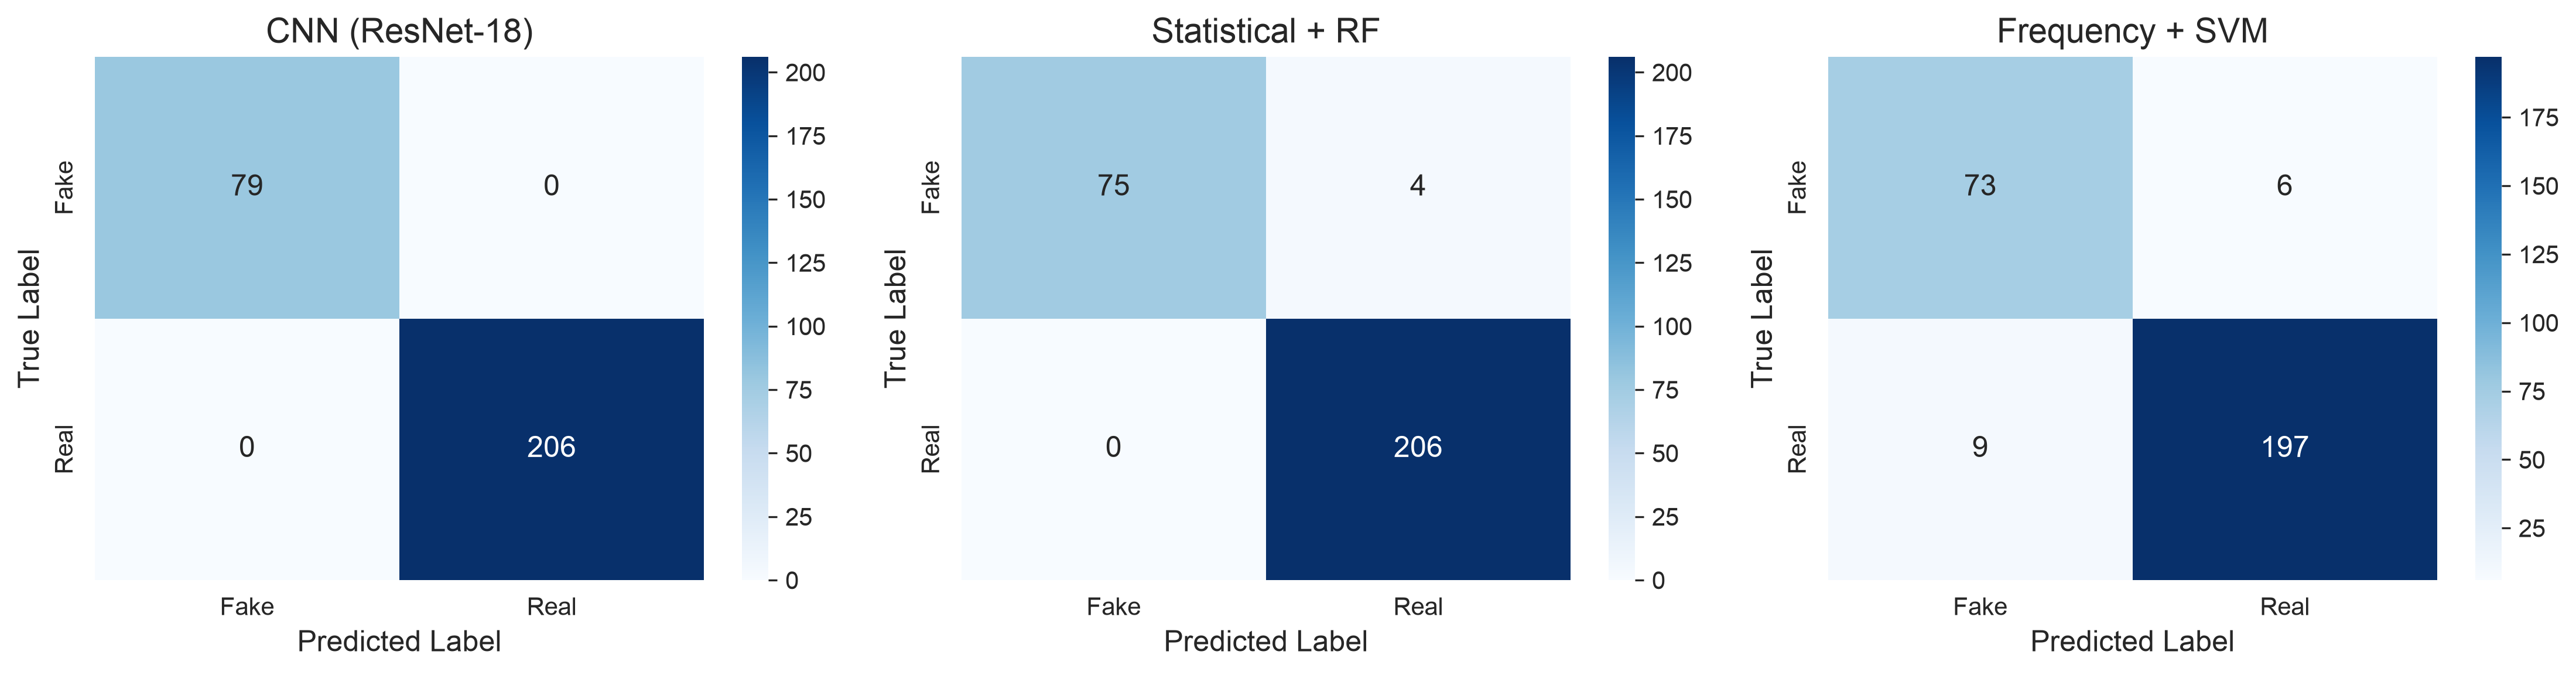
\includegraphics[width=\linewidth]{../results/figures/confusion_matrices.png}
\caption{Confusion matrices for each detector and the ensemble on the test set.}
\label{fig:confusion}
\end{figure}

\begin{figure}[h]
\centering
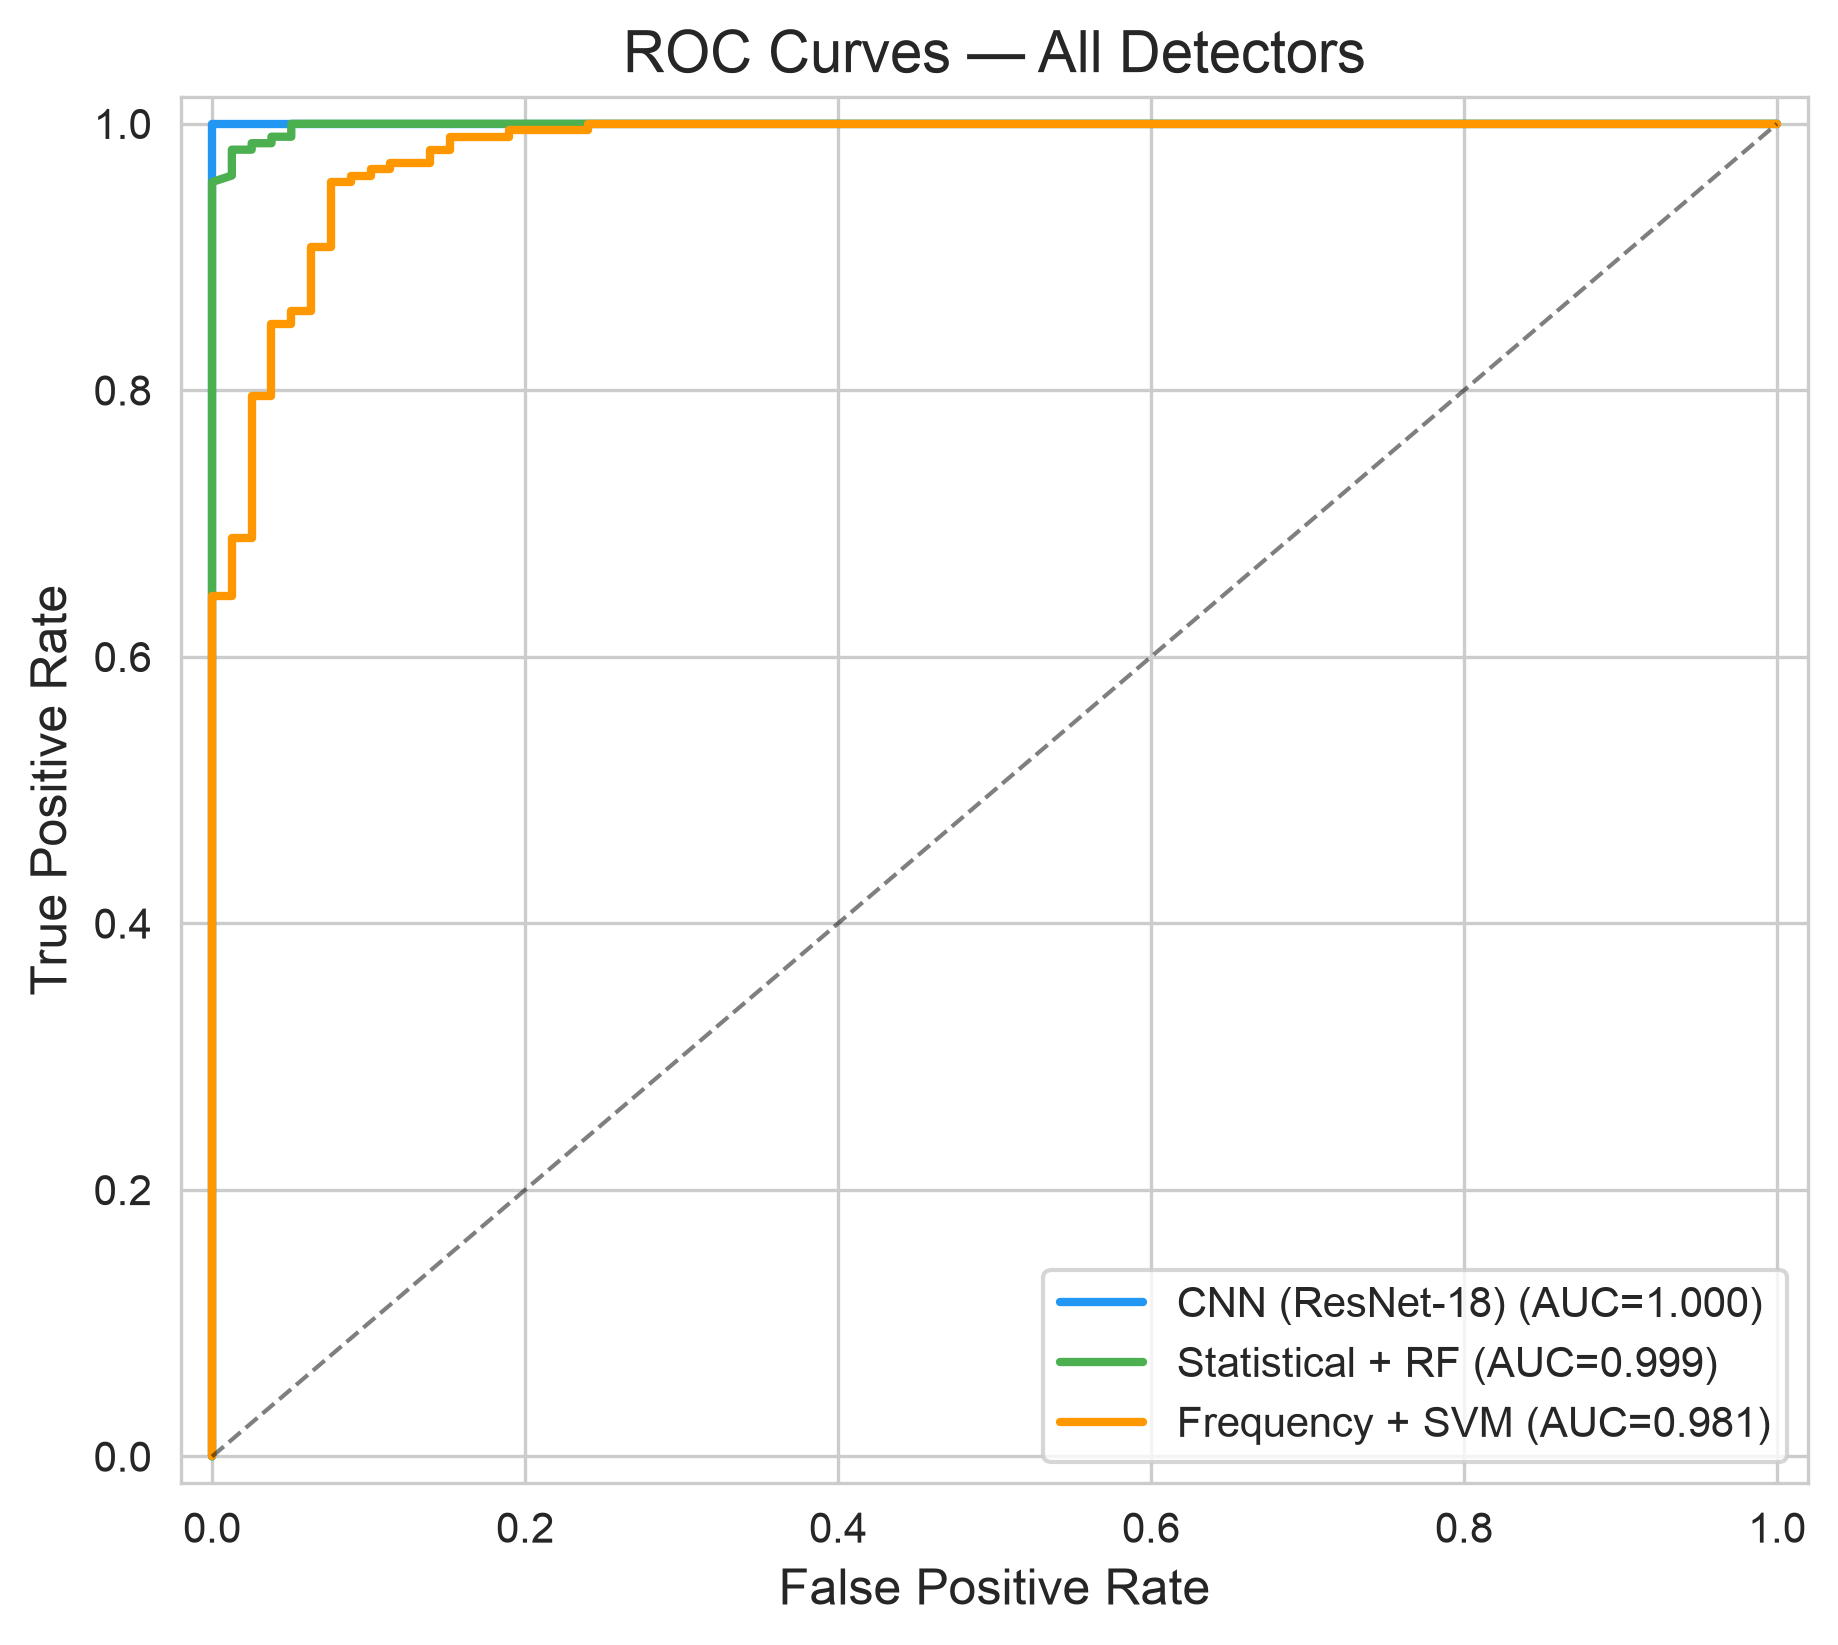
\includegraphics[width=0.8\linewidth]{../results/figures/roc_curves.png}
\caption{ROC curves comparing detector discrimination ability.}
\label{fig:roc}
\end{figure}

\subsection{Impact of Generation Method}

A key finding is that different fake generation methods have varying impacts on detector performance. Table~\ref{tab:impact} compares F1 scores when the test set contains only code-level fakes versus both types.

\begin{table}[h]
\centering
\caption{Impact of pixel-level fakes on detection F1 score.}
\label{tab:impact}
\begin{tabular}{lccc}
\toprule
\textbf{Method} & \textbf{Code Only} & \textbf{Code + Pixel} & \textbf{$\Delta$F1} \\
\midrule
Frequency + SVM & 0.960 & 0.930 & $-$0.030 \\
Statistical + RF & 0.979 & 0.972 & $-$0.007 \\
CNN (ResNet-18) & 1.000 & 0.988 & $-$0.012 \\
\bottomrule
\end{tabular}
\end{table}

Several observations emerge:

\textbf{Code-level fakes are easy to detect.} When the test set contains only code-generated figures, the CNN achieves perfect detection. This is expected: matplotlib-rendered images have characteristic properties (specific font rendering, anti-aliasing patterns, fixed DPI) that differ from figures extracted from PDFs.

\textbf{Pixel-level fakes are harder.} Adding Stable Diffusion-generated figures reduces performance across all detectors, with frequency analysis most affected ($-$3.0\% F1). Pixel-level fakes bypass the code rendering pipeline entirely, producing images with different artifact patterns.

\textbf{Statistical features are most robust.} The handcrafted statistical features show the smallest performance drop ($-$0.7\%), suggesting they capture generation-agnostic artifacts such as inconsistent edge patterns, unusual color distributions, and layout irregularities.

\subsection{CNN Training Dynamics}

The ResNet-18 converges rapidly, reaching 98\% training accuracy by epoch 3 and stabilizing at 98.6\% validation F1 by epoch 8. The fast convergence suggests that the real-vs-fake distinction is well-captured by pretrained ImageNet features, requiring only fine-tuning of the classification head.

\subsection{Feature Importance Analysis}

The Random Forest feature importance analysis reveals that the most discriminative statistical features are:
\begin{enumerate}
    \item Color diversity ratio (Feature 17) --- AI-generated charts tend to use simpler color palettes
    \item White background ratio (Feature 23) --- real extracted figures often have compression artifacts reducing pure white regions
    \item Laplacian statistics (Features 15, 18) --- differences in sharpness and edge rendering
    \item Noise patterns (Feature 35) --- AI-generated images exhibit different noise characteristics
\end{enumerate}

\section{Discussion}

\textbf{Implications for Scientific Integrity.} Our results demonstrate that current AI-generated scientific figures are detectable with high accuracy, but the gap between code-level and pixel-level detection suggests this will become harder as generation models improve. The fact that frequency analysis is most affected by pixel-level fakes indicates that generative models are learning to produce more realistic spectral properties.

\textbf{Limitations.} Our dataset, while sufficient for demonstrating the detection pipeline, is limited in scale (442 fake figures). The pixel-level fakes are generated by a single model (SD v1.5); newer models like SDXL or DALL-E 3 may produce harder-to-detect figures. Additionally, our detectors are trained on ML-domain charts and may not generalize to other scientific disciplines.

\textbf{Adversarial Robustness.} We do not evaluate adversarial attacks where a generator is specifically optimized to evade our detectors. This cat-and-mouse dynamic is an important direction for future work.

\textbf{Future Work.} We identify several directions: (1) scaling the dataset with more generation models, (2) per-chart-type analysis of detection difficulty, (3) cross-domain evaluation on figures from biology, physics, and chemistry papers, and (4) integration with existing scientific integrity tools.

\section{Conclusion}

We present a comprehensive pipeline for detecting AI-generated scientific figures, addressing a growing concern in research integrity. Our dataset construction methodology---combining arXiv scraping, CLIP-based filtering, and two distinct fake generation pathways---provides a foundation for future research. The comparison of three detection methods reveals that while CNN-based approaches achieve the highest accuracy, handcrafted statistical features offer the best robustness across generation methods. As generative models continue to improve, maintaining effective detection capabilities will require ongoing research and larger, more diverse datasets.

\section*{Code and Data Availability}

All code, trained models, and generation pipelines are available at:
\url{https://github.com/zyx100089-eng/ai-figure-detector}

\bibliographystyle{plainnat}
\bibliography{references}

\end{document}
